% !TeX spellcheck = en_EN-English
\documentclass[a4paper]{article}
\usepackage[slovak]{babel}
\usepackage[utf8]{inputenc}
\usepackage[T1]{fontenc}
\usepackage{a4wide}
\usepackage{amsmath}
\usepackage{amsfonts}
\usepackage{amssymb}
\usepackage{mathrsfs}
\usepackage[small,bf]{caption}
\usepackage{subcaption}
\usepackage{xcolor}
\usepackage{graphicx}
\usepackage{enumerate}
\usepackage{hyperref}



\pagestyle{empty}
\setlength{\parindent}{0pt}

\newenvironment{modenumerate}
{\enumerate\setupmodenumerate}
{\endenumerate}

\newif\ifmoditem
\newcommand{\setupmodenumerate}{%
	\global\moditemfalse
	\let\origmakelabel\makelabel
	\def\moditem##1{\global\moditemtrue\def\mesymbol{##1}\item}%
	\def\makelabel##1{%
		\origmakelabel{##1\ifmoditem\rlap{\mesymbol}\fi\enspace}%
		\global\moditemfalse}%
}

\makeatletter
\def\@seccntformat#1{%
	\expandafter\ifx\csname c@#1\endcsname\c@section\else
	\csname the#1\endcsname\quad
	\fi}
\makeatother

\begin{document} 
	
\pagenumbering{arabic}
\pagestyle{plain}

\begin{center}
	\sc\large
	Umelá inteligencia - cvičenia 3
\end{center}

Autor: Marián Kravec

\section{Úloha 1}
\subsection{Časť 1}

Action: pickFromTable(X)

Precondition: handEmpty $\land$ onTable(X) $\land$ onTop(X)

Effect: holding(X) 
\\

Action: stack(X,Y)

Precondition: holding(X) $\land$ onTop(Y)

Effect: on(X,Y)
\\

Action: unstack(X,Y)

Precondition: handEmpty $\land$ onTop(X) $\land$ on(X,Y)

Effect: holding(X) $\land$ onTop(Y)
\\

Action: putOnTable(X)

Precondition: holding(X)

Effect: onTable(X)
\\

\subsection{Časť 2}

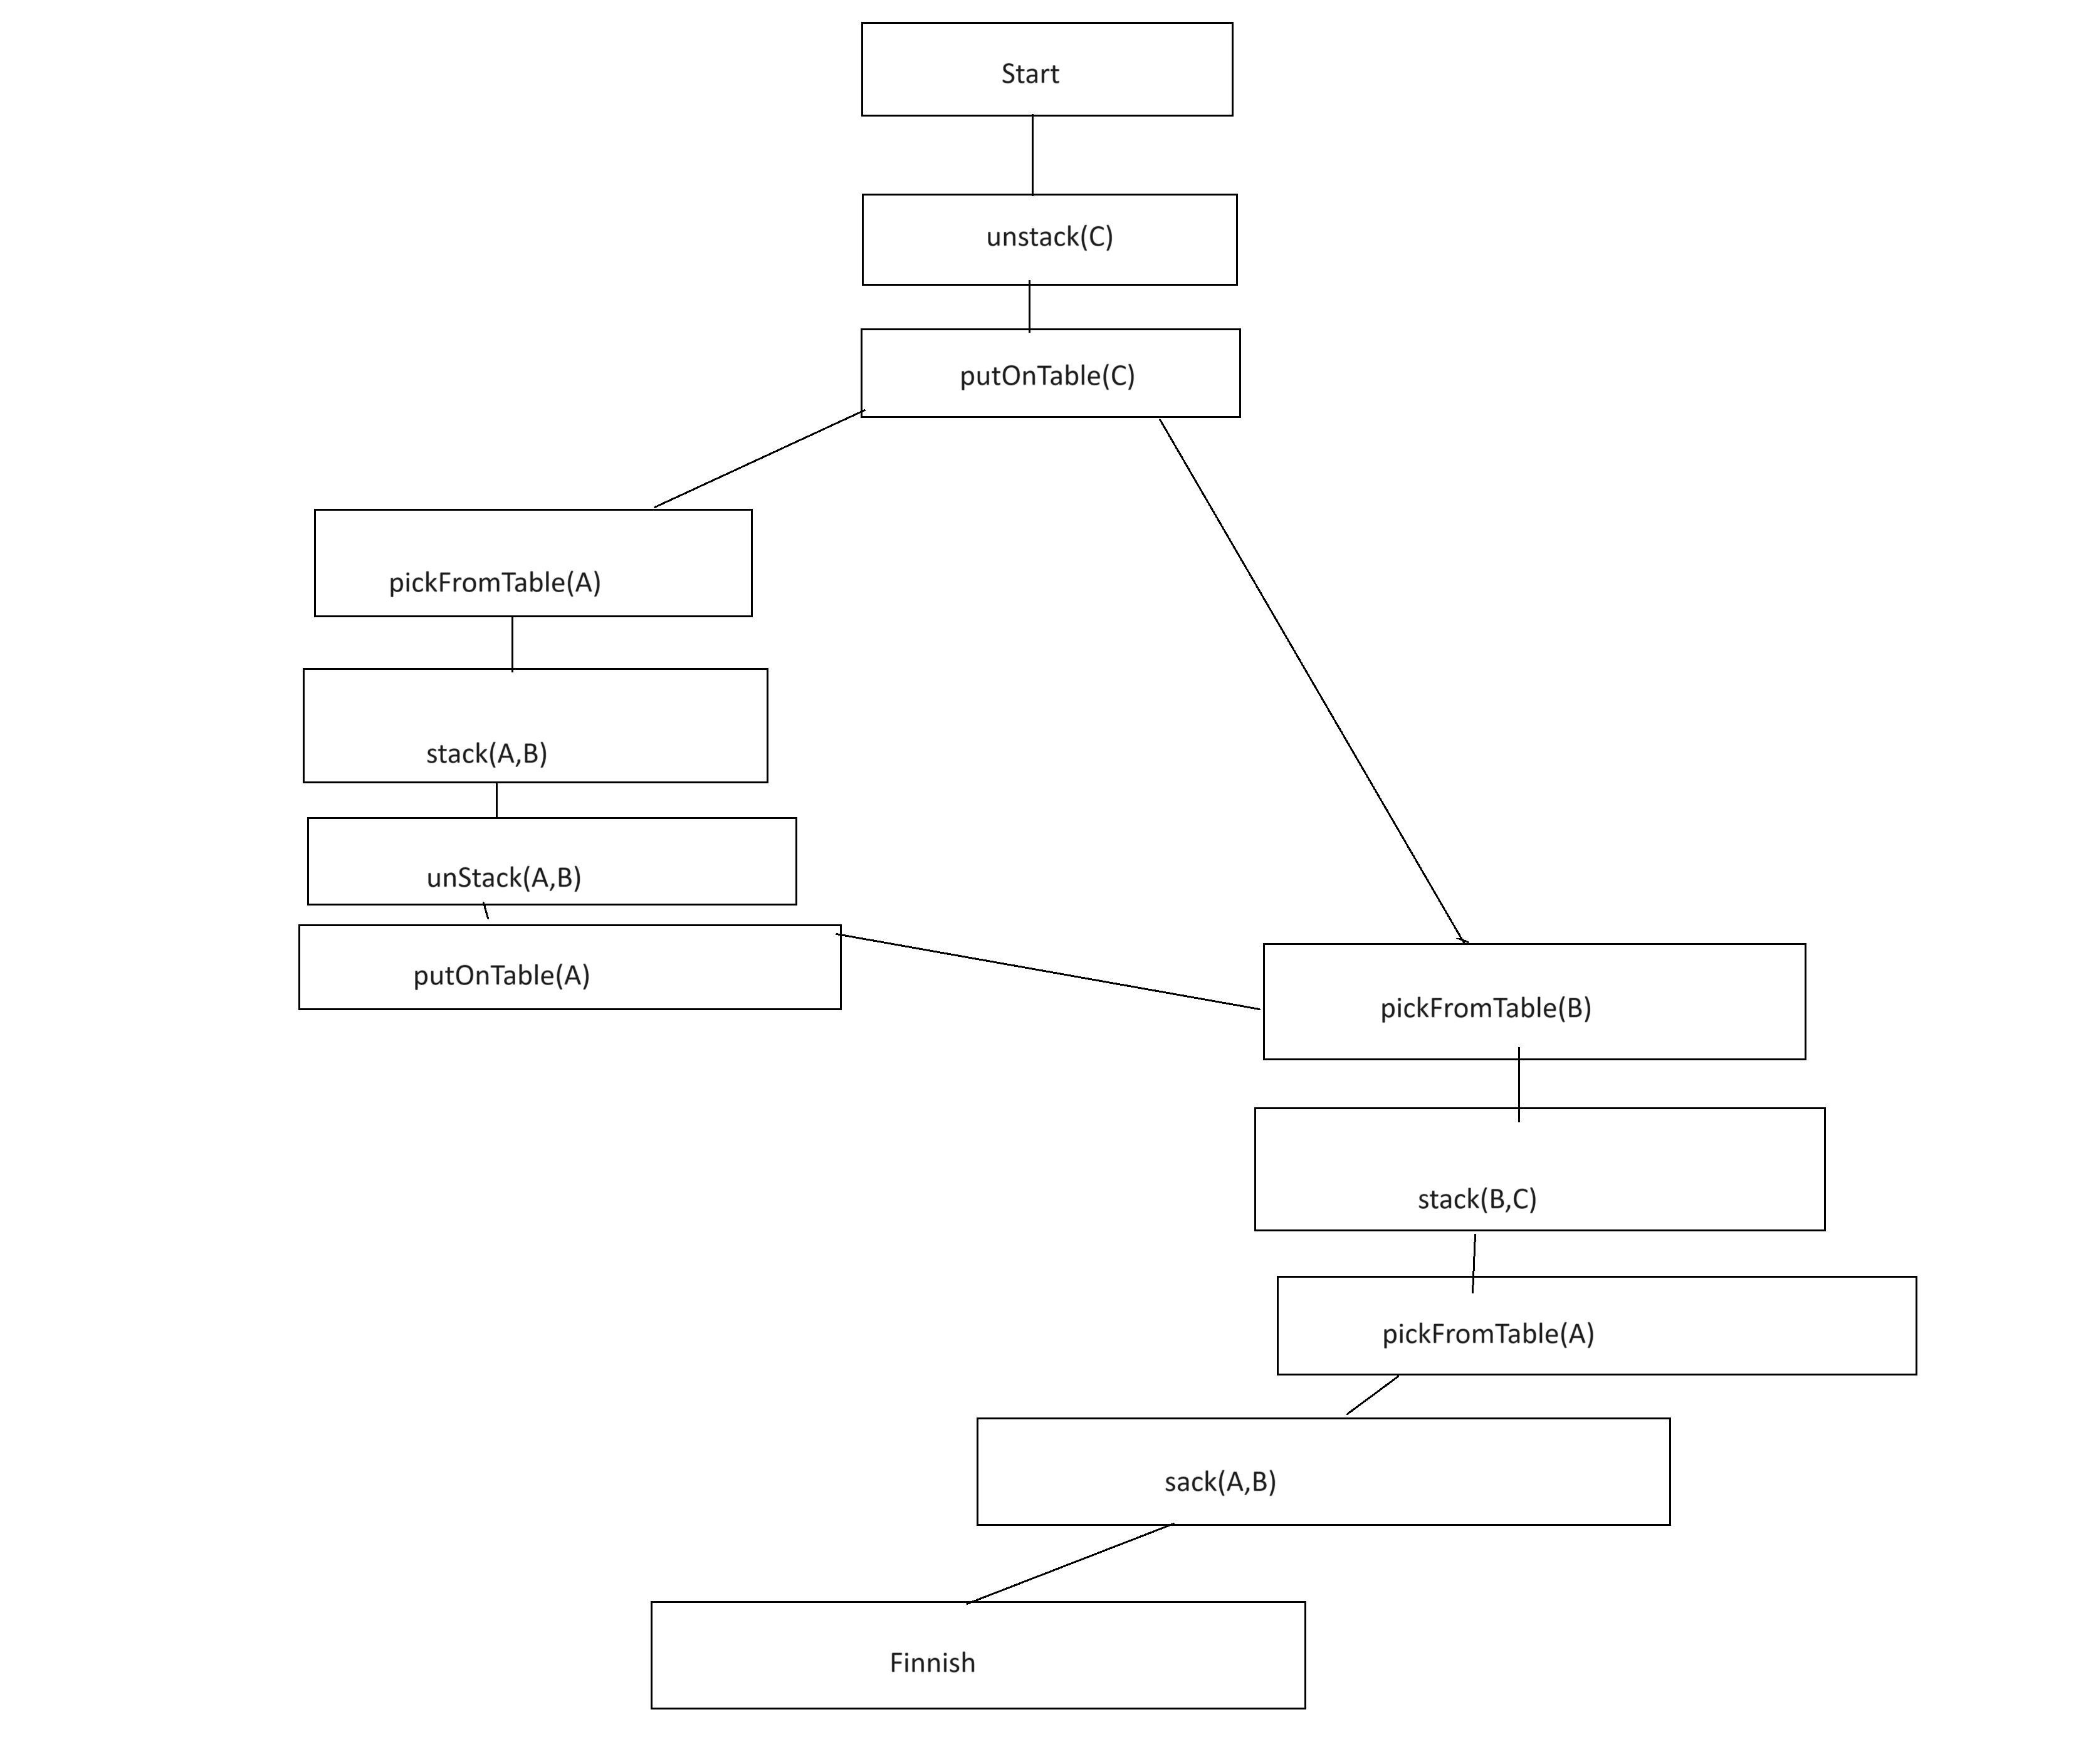
\includegraphics[width=\textwidth]{pop.png}



\end{document}